\documentclass{article}
    
    \usepackage{graphicx} % Used to insert images
    \usepackage{adjustbox} % Used to constrain images to a maximum size 
    \usepackage{color} % Allow colors to be defined
    \usepackage{enumerate} % Needed for markdown enumerations to work
    \usepackage{geometry} % Used to adjust the document margins
    \usepackage{amsmath} % Equations
    \usepackage{amssymb} % Equations
    \usepackage{eurosym} % defines \euro
    \usepackage[mathletters]{ucs} % Extended unicode (utf-8) support
    \usepackage[utf8x]{inputenc} % Allow utf-8 characters in the tex document
    \usepackage{fancyvrb} % verbatim replacement that allows latex
    \usepackage{grffile} % extends the file name processing of package graphics 
                         % to support a larger range 
    % The hyperref package gives us a pdf with properly built
    % internal navigation ('pdf bookmarks' for the table of contents,
    % internal cross-reference links, web links for URLs, etc.)
    \usepackage{hyperref}
    \usepackage{longtable} % longtable support required by pandoc >1.10
    \usepackage{booktabs}  % table support for pandoc > 1.12.2
    \usepackage{indentfirst}
    \usepackage{floatrow}
    \usepackage{relsize}
    \usepackage{multirow}
        
    \newcommand\perm[2]{{}_{#1}P_{#2}}%
    \newcommand\todo[1]{\textbf{TODO: #1}}% 
    \newcommand\numberthis{\addtocounter{equation}{1}\tag{\theequation}}
    \newcommand\seteq{\mathrel{\overset{\makebox[0pt]{\mbox{\normalfont\small\sffamily set}}}{=}}}
    \newcommand\mfrac[2]{\left(\dfrac{#1}{#2}\right)}
    \newcommand\lint{\mathlarger{\int}}
    \newcommand\lsum{\mathlarger{\sum}}
    
    \title{Homework 12}
    \author{Roly Vicar\'ia \\ STAT414 Spring 2016}
    
\begin{document}
    
    \maketitle
    
    \textbf{Section 4.5}
    \begin{enumerate}
     %1
     \item 
      \begin{enumerate}
       %a
       \item
	\begin{align*}
	 P(-5 < X < 5) &= P\left(\dfrac{-5 - (-3)}{5} < \dfrac{X - (-3)}{5} < \dfrac{5 - (-3)}{5}\right) \\
	  &= \Phi\mfrac{8}{5} - \Phi\mfrac{-2}{5} \\
	  &= .9452 - .3446 = 0.6006
	\end{align*}
       
       %b
       \item
	The conditional pdf of $X$, given that $Y=13$, is normal with mean, 
	$$\mu_X + \rho \mfrac{\sigma_X}{\sigma_Y}(y - \mu_Y)$$
	$$-3 + \mfrac{3}{5}\mfrac{5}{3}(13 - 10) = 0$$
	and variance,
	$$\sigma_X^2(1 - \rho^2)$$
	$$25\left(1 - \mfrac{3}{5}^2\right) = 16$$
	
	Therefore,
	\begin{align*}
	 P(-5 < X < 5|Y=13) &= P\left(\dfrac{-5 - 0}{4} < \dfrac{X-0}{4} < \dfrac{5-0}{4}\ \Big|Y=13\right) \\
	  &= \Phi\mfrac{5}{4} \Phi\mfrac{-5}{4} = 0.8944 - 0.1056 = 0.7888
	\end{align*}
       
       %c
       \item
	\begin{align*}
	 P(7 < Y < 16) &= P\left(\dfrac{7-10}{3} < \dfrac{Y-10}{3} < \dfrac{16-10}{3}\right) \\
	  &= \Phi(2) - \Phi(-1) \\
	  &= 0.9772 - 0.1587 = 0.8185
	\end{align*}
       
       %d
       \item
	The conditional pdf of $Y$, given that $X=2$, is normal with mean,
	$$10 + \mfrac{3}{5}\mfrac{3}{5}(2 - (-3)) = 11.8$$
	and variance,
	$$9\left(1 - \mfrac{3}{5}^2\right) = 5.76$$
	
	Therefore,
	\begin{align*}
	 P(7<Y<16 | X=2) &= P\left(\dfrac{7-11.8}{2.4} < \dfrac{Y-11.8}{2.4} < \dfrac{16-11.8}{2.4}\ \Big|X=2\right) \\
	  &= \Phi(1.75) - \Phi(-2) \\
	  &= 0.9599 - 0.0228 = 0.9371
	\end{align*}
      \end{enumerate}

     
     %2
     \item
      We have that 
      $$h(y|x) = \dfrac{1}{\sigma_Y\sqrt{2\pi}\sqrt{1-\rho^2}}exp\left[-\dfrac{[y-\mu_Y - \rho(\sigma_Y/\sigma_X)(x-\mu_X)]^2}{2\sigma_Y^2(1-\rho^2)}\right]$$
      
      and that
      $$f_X(x) = \dfrac{1}{\sigma_X\sqrt{2\pi}}exp\left[-\dfrac{(x-\mu_X)^2}{2\sigma_X^2}\right]$$
      
      To add the exponents on $e$, we start by expanding out the numerator of the first,
      \begin{align*}
	[y-\mu_Y - \rho(\sigma_Y/\sigma_X)(x-\mu_X)]^2 &= 
	y^2 - 2y\mu_Y - 2y\rho\mfrac{\sigma_Y}{\sigma_X}(x-\mu_X) + 2\mu_Y\rho\mfrac{\sigma_Y}{\sigma_X}(x-\mu_X) \\
	&+ \mu_Y^2 + \rho^2\mfrac{\sigma_Y}{\sigma_X}^2(x-\mu_X)^2
      \end{align*}
      
      \todo{come back to this}
      
      We now have to add the exponents on $e$:
      \begin{align*}
       &-\dfrac{[y-\mu_Y - \rho(\sigma_Y/\sigma_X)(x-\mu_X)]^2}{2\sigma_Y^2(1-\rho^2)} - \dfrac{(x-\mu_X)^2}{2\sigma_X^2} 
      \end{align*}

     \addtocounter{enumi}{1}
     
     %4
     \item
      \begin{enumerate}
       %a
       \item
	$E(Y|X=72) = 80 + \mfrac{5}{13}\mfrac{13}{10}(72-70) = 81$
       
       %b
       \item
	$Var(Y|X=72) = 169\left(1-\mfrac{5}{13}^2\right) = 144$
       
       %c
       \item
	$P(Y \le 84|X=72) = P\left(\dfrac{Y-81}{12} \le \dfrac{84-81}{12}\ \Big|X=72\right)
	  = \Phi\mfrac{1}{4} = 0.5987$
      \end{enumerate}
     \addtocounter{enumi}{2}
     
     %7
     \item
      \begin{enumerate}
       %a
       \item
	\begin{align*}
	 P(309.2 < Y <380.6) &= P\left(\dfrac{309.2 - 347}{\sqrt{689}} < \dfrac{Y-347}{\sqrt{689}} < \dfrac{380.6 - 347}{\sqrt{689}}\right) \\
	  &= \Phi(1.28) - \Phi(-1.44) \\
	  &= 0.8997 - 0.0749 = 0.8248
	\end{align*}
       
       %b
       \item
	$E(Y|x) = 347 + (-0.25)\mfrac{\sqrt{689}}{\sqrt{611}}(x-415) 
	  = 347 + \sqrt{\dfrac{53}{47}}\left(103.75 - \dfrac{x}{4}\right)$
       
       %c
       \item
	$Var(Y|x) = 689(1 - (-0.25)^2) = 645.9375$
       
       %d
       \item
	The mean of $Y$, given that $X=385.1$, is
	$$347 + \sqrt{\dfrac{53}{47}}\left(103.75 - \dfrac{385.1}{4}\right) = 354.9378$$
	and the variance of $Y$, given that $X=385.1$, is
	$$645.9375$$
	
	Therefore,
	\begin{align*}
	 P(309.2 < Y < 380.6 | X=385.1) &= P\left(\dfrac{309.2 - 354.9378}{25.4153} < \dfrac{Y-354.9378}{25.4153} < \dfrac{380.6-354.9378}{25.4153}\right) \\
	  &= \Phi(1.0097) - \Phi(-1.7996) \\
	  &= 0.8438 - 0.0359 = 0.8079
	\end{align*}
      \end{enumerate}
     \addtocounter{enumi}{1}
     
     \newpage
     %9
     \item
      Plot of $E(Y|x) = x-3$ as well as lines 2 standard deviations above and below: $a(x) = x-11$ and 
      $b(x) = x+5$.
      \begin{figure}[h!]
	\centering
	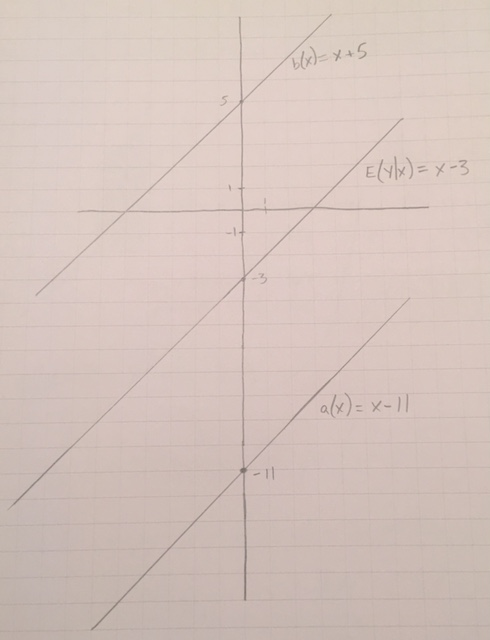
\includegraphics[scale=.6,keepaspectratio=true]{./images/Plot.jpg}
	% Plot.jpg: 490x640 pixel, 72dpi, 17.29x22.58 cm, bb=0 0 490 640
      \end{figure}
    \end{enumerate}
    
    \newpage
    \textbf{Section 5.1}
    \begin{enumerate}
     \addtocounter{enumi}{3}
     %4
     \item 
      \begin{enumerate}
       %a
       \item
	$F(x) = \lint_0^x{2t\ dt} = x^2$ for $0 < x < 1$
       
       %b
       \item
	We can simulate observations of $X$, by first defining $X=F^{-1}(Y) = \sqrt{Y}$, which maps value between
	0 and 1 to a value of $X$. Therefore, we just need to generate random numbers between 0 and 1
	and map them back to $X$ values.
       
       %c
       \item
	10 simulated observations of X:
	\begin{center}
	  \begin{tabular}{c | c}
	    Random number from $U(0,1)$ (Y) & $X = \sqrt{Y}$ \\
	    \hline
	    0.620355281478075 & 0.787626359054898 \\
	    0.146449663756424 & 0.382687423044479 \\
	    0.204920874838681 & 0.45268186935052 \\
	    0.238088079073957 & 0.487942700605263 \\
	    0.433341992859133 & 0.658287165953532 \\
	    0.306541892458699 & 0.553662254861842 \\
	    0.829008233873843 & 0.910498892846028 \\
	    0.84479018798775 & 0.919124685767796 \\
	    0.502745995936653 & 0.709045834863059 \\
	    0.708640141413394 & 0.841807662957159 
	  \end{tabular}
	\end{center}
      \end{enumerate}
     
     %5
     \item
      We are given that $f(x) = \theta x^{\theta - 1}$ for $0 < x < 1, 0 < \theta < \infty$. And 
      $Y=-2\theta \ln{X}$. 
      
      From this we compute $v(y) = X = e^{-y/2\theta}$. 
      
      Then we compute the derivative, $v'(y) = -\dfrac{1}{2\theta}e^{-y/2\theta}$
      
      We then have that 
      \begin{align*}
       g(y) &= f[v(y)]\cdot |v'(y)| \\
	&= \theta (e^{-y/2\theta})^{\theta-1}\dfrac{1}{2\theta}e^{-y/2\theta} \\
	&= \dfrac{1}{2}\exp\left[\dfrac{-\theta y + y}{2\theta} + \dfrac{-y}{2\theta}\right] \\
	&= \dfrac{1}{2}\exp\left[-\dfrac{\theta y}{2\theta}\right] \\
	&= \dfrac{1}{2}e^{-y/2}
      \end{align*}
      
      Therefore, Y follows an exponential distritbution with mean 2.
     
     %6
     \item
      \todo{come back to this}
     \addtocounter{enumi}{3}
     
     %10
     \item
      We start by breaking up the function into two parts. When $0 < y < 1$, we have, 
      $x_1 = -\sqrt{y}$ for $-1 < x < 0$, and $x_2 = \sqrt{y}$ for $0 < x < 1$.
      
      We compute the derivatives,
      $$\dfrac{dx_1}{dy} = -\dfrac{1}{2\sqrt{y}}$$
      and
      $$\dfrac{dx_2}{dy} = \dfrac{1}{2\sqrt{y}}$$
      
      Therefore,
      \[ g(y) = 
	  \begin{cases}
	    \dfrac{1}{4} \Big|\dfrac{-1}{2\sqrt{y}}\Big| + \dfrac{1}{4} \Big|\dfrac{1}{2\sqrt{y}}\Big| 
	    = \dfrac{1}{4\sqrt{y}} & 0 < y < 1 \\
	    \dfrac{1}{4} \Big|\dfrac{1}{2\sqrt{y}}\Big| = \dfrac{1}{8\sqrt{y}} & 1 < y < 3
         \end{cases}
      \]
     \addtocounter{enumi}{3}
     
     %14
     \item
      We break up the function into two parts, $x_1 = -y$ for $-\infty < x_1 < 0$, and $x_2 = y$
      for $0 < x_1 < \infty$.
      
      We compute the derivatives,
      $$\dfrac{dx_1}{dy} = -1$$
      and
      $$\dfrac{dx_2}{dy} = 1$$
      
      Therefore,
      \begin{align*}
       g(y) &= \dfrac{1}{\sqrt{2\pi}}\exp\left[-\dfrac{(-y)^2}{2}\right]\cdot -1 + 
	\dfrac{1}{\sqrt{2\pi}}\exp\left[-\dfrac{(y)^2}{2}\right]\cdot 1 \\
	&= \dfrac{1}{\sqrt{2\pi}} \left\{\exp\left[-\dfrac{y^2}{2}\right] - \exp\left[-\dfrac{y^2}{2}\right]\right\} \\
	&= 0
      \end{align*}
    \end{enumerate}

    \textbf{Section 5.2}
    \begin{enumerate}
     \addtocounter{enumi}{3}
     %4
     \item 
      \begin{enumerate}
       %a
       \item
	$F_{0.05}(9,24) = 2.30$
       
       %b
       \item
	$F_{0.95}(9,24) = \dfrac{1}{F_{0.05}(24,9)} = \dfrac{1}{2.90} = 0.3448$
       
       %c
       \item
	$P(0.277 \le W \le 2.70) = 0.9498$
      \end{enumerate}
     \addtocounter{enumi}{3}
     
     %8
     \item
      \todo{come back to this}
      \begin{enumerate}
       %a
       \item
	
       
       %b
       \item
      \end{enumerate}

     
     %9
     \item
      $c = \dfrac{\Gamma(11)}{\Gamma(4)\Gamma(7)} = 840$
     \addtocounter{enumi}{1}
     
     %11
     \item
      \begin{enumerate}
       %a
       \item
	\begin{align*}
	 \lint_0^{0.4} {\dfrac{\Gamma(7)}{\Gamma(4)\Gamma(3)}y^3(1-y)^2\ dy} 
	 &= \dfrac{\Gamma(7)}{\Gamma(4)\Gamma(3)} \lint_0^{0.4}{y^3(1-y)^2\ dy} \\
	 &= \dfrac{\Gamma(7)}{\Gamma(4)\Gamma(3)} \lint_0^{0.4}{y^3 - 2y^4 + y^5\ dy} \\
	 &= \dfrac{\Gamma(7)}{\Gamma(4)\Gamma(3)} \left[\dfrac{y^4}{4} - \dfrac{2y^5}{5} + \dfrac{y^6}{6} \right]_0^{0.4} \\
	 &= \dfrac{\Gamma(7)}{\Gamma(4)\Gamma(3)} (0.002987) \\
	 &= 0.1792
	\end{align*}
       
       %b
       \item
	\begin{align*}
	 \lsum_{y=4}^{6} {\dbinom{6}{y}(0.4)^y(0.6)^{6-y}} 
	 &= \dbinom{6}{4}(0.4)^4(0.6)^{2} + \dbinom{6}{5}(0.4)^5(0.6)^{1} + \dbinom{6}{6}(0.4)^6(0.6)^{0} \\ 
	 &= 0.13824 + 0.03686 + 0.004096 \\
	 &= 0.1792
	\end{align*}
      \end{enumerate}
    \end{enumerate}
\end{document}